\documentclass[12pt,a4paper]{article}

\usepackage[T1]{fontenc}
\usepackage[utf8]{inputenc}
\usepackage[brazil]{babel}
\usepackage[a4paper,margin=2.5cm]{geometry}
\usepackage{graphicx}
\usepackage{array}
\usepackage{longtable}
\usepackage{booktabs}
\usepackage{float}
\usepackage{amsmath}
\usepackage{hyperref}
\usepackage{enumitem}

\hypersetup{
    colorlinks=true,
    linkcolor=black,
    urlcolor=blue
}

\setlist[itemize]{leftmargin=1.5cm}
\setlist[enumerate]{leftmargin=1.2cm}

\newcommand{\placeholderfigure}[2]{
\begin{figure}[H]
\centering
\fbox{
\parbox[c][#2][c]{0.85\textwidth}{
\centering
\textbf{Placeholder para imagem}\\[0.5em]
#1
}
}
\caption{#1}
\end{figure}
}

\title{\textbf{Estudo Dirigido 01 -- Pizzaria Ca\'otica}\\[0.5em]
\large Documenta\c{c}\~ao do C\'odigo e Estrutura do Projeto}
\author{
    CC7N
Rafael Wernesbach\\
Rafael Bassul\\
}
\date{\today}

\begin{document}

\maketitle

\section{Introdu\c{c}\~ao}
Este documento apresenta a documenta\c{c}\~ao completa do projeto da pizzaria concorrente, seguindo a organiza\c{c}\~ao solicitada no PDF da atividade. O c\'odigo foi dividido em quatro arquivos principais:
\texttt{main.py}, \texttt{pizzaria.py}, \texttt{interface.py} e \texttt{graph.py}. Em conjunto, esses arquivos implementam a simula\c{c}\~ao da produ\c{c}\~ao e entrega de pizzas com m\'ultiplas threads, controle de recurso limitado por sem\'aforo, sincroniza\c{c}\~ao por condi\c{c}\~ao e visualiza\c{c}\~ao do estado da execu\c{c}\~ao.

O projeto modela um cen\'ario produtor-consumidor em que chefs produzem pizzas premium a partir da busca por n\'umeros primos grandes, enquanto entregadores consomem os pedidos prontos e realizam a entrega. Al\'em da simula\c{c}\~ao, o projeto tamb\'em possui uma interface gr\'afica para acompanhar o estado interno e um script separado para medi\c{c}\~ao de desempenho e gera\c{c}\~ao de gr\'aficos.

\section{Vis\~ao Geral da Arquitetura}
\begin{longtable}{>{\raggedright\arraybackslash}p{0.22\textwidth} >{\raggedright\arraybackslash}p{0.72\textwidth}}
\toprule
\textbf{Arquivo} & \textbf{Responsabilidade principal} \\
\midrule
\endhead
\texttt{main.py} & Ponto de entrada da aplica\c{c}\~ao. L\^e os par\^ametros da simula\c{c}\~ao, inicia a interface gr\'afica e dispara a execu\c{c}\~ao concorrente em uma thread separada. \\
\texttt{pizzaria.py} & N\'ucleo da l\'ogica concorrente. Define fila, sem\'aforo, condi\c{c}\~ao, estado compartilhado, fun\c{c}\~oes auxiliares e as classes \texttt{Chef} e \texttt{Entregador}. \\
\texttt{interface.py} & Implementa a interface em Tkinter, exibindo em tempo real o estado dos chefs, dos entregadores e das estat\'isticas gerais da simula\c{c}\~ao. \\
\texttt{graph.py} & Executa a simula\c{c}\~ao em diferentes configura\c{c}\~oes, mede o tempo total de execu\c{c}\~ao, calcula o speedup e gera os gr\'aficos de desempenho. \\
\bottomrule
\end{longtable}

\section{Etapa 1 -- Planejamento e Defini\c{c}\~ao do Problema}

\subsection{Entrada do sistema}
As entradas principais do sistema s\~ao:
\begin{itemize}
    \item quantidade de chefs;
    \item quantidade de entregadores;
    \item quantidade de pizzas que cada chef deve produzir.
\end{itemize}

Esses valores s\~ao lidos no arquivo \texttt{main.py} por meio do terminal, antes da cria\c{c}\~ao da interface gr\'afica e do in\'icio da simula\c{c}\~ao.

\subsection{Sa\'ida esperada}
As sa\'idas esperadas do sistema s\~ao:
\begin{itemize}
    \item mensagens no terminal indicando a produ\c{c}\~ao e a entrega das pizzas;
    \item atualiza\c{c}\~ao visual em tempo real da situa\c{c}\~ao dos chefs e entregadores na interface gr\'afica;
    \item medi\c{c}\~oes de tempo de execu\c{c}\~ao e speedup no script \texttt{graph.py};
    \item um gr\'afico comparando tempo total e speedup em fun\c{c}\~ao do n\'umero de threads.
\end{itemize}

\subsection{Recursos limitados}
O principal recurso limitado do sistema \'e o forno, modelado por um sem\'aforo. Na implementa\c{c}\~ao atual, o forno foi criado com:
\begin{center}
\texttt{threading.Semaphore(2)}
\end{center}
Isso significa que apenas dois chefs podem usar o forno simultaneamente. O PDF sugere o uso de \texttt{Semaphore(3)}; portanto, a vers\~ao atual est\'a conceitualmente correta, mas com uma capacidade diferente da sugerida no enunciado.

\subsection{Produtores, consumidores e fila}
Os produtores s\~ao os chefs, pois geram pizzas e colocam os pedidos prontos na fila compartilhada. Os consumidores s\~ao os entregadores, que retiram pizzas da fila e simulam a entrega.

Na implementa\c{c}\~ao atual, a fila foi criada como:
\begin{center}
\texttt{Queue(maxsize=100)}
\end{center}
O enunciado sugere uma fila na faixa de 30 a 50 itens. Assim, o projeto j\'a utiliza uma fila limitada, mas o valor atual pode ser ajustado caso seja necess\'ario aderir de forma literal \`a recomenda\c{c}\~ao do PDF.

\subsection{Configura\c{c}\~oes de teste}
Para atender ao enunciado, as configura\c{c}\~oes m\'inimas recomendadas para medi\c{c}\~ao s\~ao:
\begin{itemize}
    \item 1 chef + 1 entregador;
    \item 2 chefs + 2 entregadores;
    \item 4 chefs + 4 entregadores;
    \item 8 chefs + 8 entregadores, ou o m\'aximo suportado pela m\'aquina.
\end{itemize}

O arquivo \texttt{graph.py} j\'a automatiza os testes de desempenho exatamente nas combina\c{c}\~oes pedidas no PDF. Na vers\~ao atual, o script executa as configura\c{c}\~oes \(1{+}1\), \(2{+}2\), \(4{+}4\) e \(8{+}8\), sempre somando chefs e entregadores para calcular o total de threads analisado nos gr\'aficos. Para que a compara\c{c}\~ao de speedup seja justa, o experimento mant\'em fixa a carga total de trabalho em 120 pizzas, distribuindo essa quantidade entre os chefs de cada teste.

\subsection{Mecanismos de sincroniza\c{c}\~ao}
Os mecanismos de sincroniza\c{c}\~ao adotados no projeto s\~ao:
\begin{itemize}
    \item \textbf{Semaphore}: usado para controlar o acesso concorrente ao forno;
    \item \textbf{Condition}: usado para coordenar a comunica\c{c}\~ao entre chefs e entregadores quando uma pizza fica pronta e \'e inserida na fila;
    \item \textbf{Lock}: usado para proteger o dicion\'ario de estado compartilhado que abastece a interface.
\end{itemize}

\section{Etapa 2 -- Implementa\c{c}\~ao}
Esta etapa documenta detalhadamente cada arquivo do projeto, explicando seu papel, suas estruturas internas e a forma como eles se relacionam.

\subsection{\texttt{main.py}}
O arquivo \texttt{main.py} funciona como ponto de entrada da aplica\c{c}\~ao. Ele organiza a inicializa\c{c}\~ao do sistema e garante que a interface gr\'afica e a simula\c{c}\~ao concorrente funcionem ao mesmo tempo.

\subsubsection{Importa\c{c}\~oes}
Esse arquivo importa:
\begin{itemize}
    \item \texttt{tkinter} para a cria\c{c}\~ao da janela principal;
    \item \texttt{Interface} do arquivo \texttt{interface.py};
    \item \texttt{iniciar\_simulacao} do arquivo \texttt{pizzaria.py};
    \item \texttt{threading} para executar a simula\c{c}\~ao sem bloquear a interface;
    \item \texttt{signal} e \texttt{sys} para tratar interrup\c{c}\~ao por teclado.
\end{itemize}

\subsubsection{Fun\c{c}\~ao \texttt{signal\_handler}}
Essa fun\c{c}\~ao recebe o sinal de interrup\c{c}\~ao e encerra o programa de maneira simples. Ela imprime uma mensagem no terminal e chama \texttt{sys.exit(0)}.

\subsubsection{Fluxo principal}
No bloco \texttt{if \_\_name\_\_ == "\_\_main\_\_"}:
\begin{enumerate}
    \item o programa registra o tratador de \texttt{SIGINT};
    \item solicita ao usu\'ario a quantidade de chefs;
    \item solicita a quantidade de entregadores;
    \item solicita a quantidade de pizzas por chef;
    \item cria a janela principal do Tkinter;
    \item instancia a classe \texttt{Interface};
    \item cria uma thread separada para executar \texttt{iniciar\_simulacao};
    \item inicia o loop principal da interface com \texttt{root.mainloop()}.
\end{enumerate}

\subsubsection{Fun\c{c}\~ao do arquivo no sistema}
Esse arquivo faz a integra\c{c}\~ao entre interface e simula\c{c}\~ao. A decis\~ao de executar a simula\c{c}\~ao em outra thread \'e importante porque evita o travamento da interface enquanto chefs e entregadores trabalham em paralelo.

\subsection{\texttt{pizzaria.py}}
O arquivo \texttt{pizzaria.py} concentra a l\'ogica principal do projeto. Ele implementa o problema produtor-consumidor, a restri\c{c}\~ao de acesso ao forno, o acompanhamento do estado global e a cria\c{c}\~ao das threads.

\subsubsection{Estruturas globais}
As principais estruturas globais s\~ao:
\begin{itemize}
    \item \texttt{fila}: fila compartilhada de pizzas prontas;
    \item \texttt{forno}: sem\'aforo que limita quantos chefs podem usar o forno ao mesmo tempo;
    \item \texttt{condition}: vari\'avel de condi\c{c}\~ao usada para acordar entregadores quando uma pizza fica pronta;
    \item \texttt{estado\_lock}: lock que protege as altera\c{c}\~oes no dicion\'ario \texttt{estado};
    \item \texttt{estado}: dicion\'ario com dados de chefs, entregadores, quantidade na fila, pizzas produzidas e pizzas entregues;
    \item \texttt{SENTINELA}: objeto especial usado para sinalizar o encerramento dos entregadores.
\end{itemize}

\subsubsection{Fun\c{c}\~ao \texttt{eh\_primo}}
A fun\c{c}\~ao \texttt{eh\_primo(x)} verifica se um n\'umero \'e primo. O algoritmo:
\begin{itemize}
    \item rejeita valores menores que 2;
    \item trata separadamente o caso do n\'umero 2;
    \item elimina n\'umeros pares;
    \item testa divisibilidade apenas por \'impares at\'e a raiz quadrada de \texttt{x}.
\end{itemize}

No contexto da simula\c{c}\~ao, cada n\'umero primo encontrado representa uma pizza premium pronta.

\subsubsection{Fun\c{c}\~oes de atualiza\c{c}\~ao de estado}
As fun\c{c}\~oes \texttt{atualizar\_estado\_chef} e \texttt{atualizar\_estado\_entregador} atualizam o dicion\'ario compartilhado que abastece a interface. Elas registram:
\begin{itemize}
    \item o nome da thread;
    \item o status atual;
    \item a quantidade de pizzas feitas;
    \item a fila atual;
    \item contadores globais de produ\c{c}\~ao e entrega.
\end{itemize}

Essas fun\c{c}\~oes s\~ao importantes porque desacoplam a simula\c{c}\~ao da interface: a l\'ogica concorrente atualiza apenas o estado, enquanto a interface apenas o l\^e.

\subsubsection{Classe \texttt{Chef}}
A classe \texttt{Chef} herda de \texttt{threading.Thread}. Cada objeto dessa classe representa um produtor.

O m\'etodo \texttt{run()} executa o seguinte fluxo:
\begin{enumerate}
    \item marca o chef como separando ingredientes;
    \item entra em la\c{c}o at\'e produzir a quantidade desejada de pizzas;
    \item informa que est\'a esperando o forno;
    \item entra na regi\~ao protegida pelo sem\'aforo;
    \item gera um n\'umero grande aleat\'orio;
    \item testa se o n\'umero \'e primo;
    \item se for primo, registra uma pizza pronta;
    \item insere a pizza na fila compartilhada;
    \item incrementa o contador global de pizzas produzidas;
    \item chama \texttt{condition.notify()} para acordar uma thread consumidora;
    \item ao final, marca seu estado como finalizado.
\end{enumerate}

Esse comportamento representa corretamente o papel de produtor e mostra o uso combinado de sem\'aforo, fila e condi\c{c}\~ao.

\subsubsection{Classe \texttt{Entregador}}
A classe \texttt{Entregador} tamb\'em herda de \texttt{threading.Thread}. Cada inst\^ancia representa um consumidor.

O m\'etodo \texttt{run()} segue o fluxo abaixo:
\begin{enumerate}
    \item marca o entregador como ocioso;
    \item entra em um la\c{c}o infinito;
    \item espera enquanto a fila estiver vazia, usando \texttt{condition.wait()};
    \item remove uma pizza da fila quando houver item dispon\'ivel;
    \item verifica se o item recebido \'e a sentinela;
    \item se for sentinela, encerra a thread;
    \item se for pizza normal, imprime a entrega, atualiza o estado e dorme por um curto intervalo para simular o tempo de entrega;
    \item incrementa o contador de pizzas entregues e volta ao estado ocioso.
\end{enumerate}

Essa classe materializa o lado consumidor do padr\~ao produtor-consumidor.

\subsubsection{Fun\c{c}\~ao \texttt{iniciar\_simulacao}}
Essa fun\c{c}\~ao organiza toda a execu\c{c}\~ao concorrente:
\begin{enumerate}
    \item recebe as quantidades de chefs, entregadores e pizzas por chef;
    \item cria as threads correspondentes;
    \item inicia primeiro os entregadores;
    \item inicia os chefs;
    \item aguarda o t\'ermino de todos os chefs com \texttt{join()};
    \item envia uma sentinela para cada entregador;
    \item acorda todas as threads consumidoras com \texttt{condition.notify\_all()} para evitar que alguma permane\c{c}a bloqueada em \texttt{condition.wait()};
    \item aguarda o t\'ermino de todos os entregadores;
    \item retorna as listas de threads criadas.
\end{enumerate}

Essa organiza\c{c}\~ao evita deadlock no encerramento e garante que todos os entregadores terminem de forma controlada, inclusive quando alguma thread consumidora est\'a aguardando nova pizza no momento em que a produ\c{c}\~ao termina.

\subsubsection{Fun\c{c}\~ao do arquivo no sistema}
Esse \'e o arquivo mais importante do projeto, pois define a sem\^antica da concorr\^encia e a coordena\c{c}\~ao entre os componentes.

\subsection{\texttt{interface.py}}
O arquivo \texttt{interface.py} implementa a visualiza\c{c}\~ao da simula\c{c}\~ao em tempo real utilizando Tkinter.

\subsubsection{Classe \texttt{Interface}}
A classe \texttt{Interface} recebe o objeto \texttt{root} da janela principal e constr\'oi os componentes visuais.

No construtor \texttt{\_\_init\_\_}, o arquivo:
\begin{itemize}
    \item define o t\'itulo da janela;
    \item cria um r\'otulo superior para estat\'isticas gerais;
    \item cria uma \'area de texto para exibir os chefs;
    \item cria uma \'area de texto para exibir os entregadores;
    \item chama imediatamente o m\'etodo \texttt{update()}.
\end{itemize}

\subsubsection{M\'etodo \texttt{update}}
Esse m\'etodo realiza a atualiza\c{c}\~ao peri\'odica da interface:
\begin{enumerate}
    \item entra em regi\~ao protegida por \texttt{estado\_lock};
    \item copia os dados de chefs, entregadores e contadores;
    \item atualiza o r\'otulo principal com pizzas produzidas, entregues e tamanho da fila;
    \item limpa e reescreve a caixa de texto dos chefs;
    \item limpa e reescreve a caixa de texto dos entregadores;
    \item agenda uma nova atualiza\c{c}\~ao ap\'os 500 milissegundos com \texttt{root.after(500, self.update)}.
\end{enumerate}

\subsubsection{Fun\c{c}\~ao do arquivo no sistema}
Esse arquivo tem papel de monitoramento. Ele n\~ao altera a simula\c{c}\~ao, apenas consome o estado compartilhado e o apresenta de forma leg\'ivel para o usu\'ario.

\subsection{\texttt{graph.py}}
O arquivo \texttt{graph.py} foi criado para a etapa experimental da atividade, permitindo medir tempo de execu\c{c}\~ao e calcular speedup.

\subsubsection{Configura\c{c}\~ao atual}
Na vers\~ao atual do script:
\begin{itemize}
    \item a carga total do experimento foi fixada em 120 pizzas;
    \item as configura\c{c}\~oes testadas s\~ao \(1\) chef + \(1\) entregador, \(2\) chefs + \(2\) entregadores, \(4\) chefs + \(4\) entregadores e \(8\) chefs + \(8\) entregadores;
    \item a quantidade de pizzas por chef \'e calculada a partir dessa carga total, resultando em 120, 60, 30 e 15 pizzas por chef, respectivamente;
    \item o tempo de execu\c{c}\~ao \'e medido com \texttt{timeit.default\_timer()};
    \item o gr\'afico final \'e salvo automaticamente no arquivo \texttt{grafico\_pizzaria.png};
    \item o script trata interrup\c{c}\~ao por teclado com \texttt{KeyboardInterrupt};
    \item ao final, o terminal exibe uma tabela textual com configura\c{c}\~ao, total de threads, pizzas por chef, pizzas totais, tempo e speedup.
\end{itemize}

\subsubsection{Fluxo do script}
O script realiza os seguintes passos:
\begin{enumerate}
    \item define uma lista fixa de configura\c{c}\~oes de teste no formato \((chefs, entregadores)\);
    \item calcula automaticamente quantas pizzas cada chef dever\'a produzir, mantendo o total de 120 pizzas em todas as execu\c{c}\~oes;
    \item reinicializa o estado compartilhado antes de cada teste;
    \item imprime no terminal uma mensagem de in\'icio para cada experimento;
    \item mede o tempo total da simula\c{c}\~ao;
    \item armazena o tempo obtido;
    \item calcula o speedup em rela\c{c}\~ao ao primeiro teste, que \'e a configura\c{c}\~ao base \(1\) chef + \(1\) entregador;
    \item imprime uma tabela final com os valores exatos medidos;
    \item gera dois subgr\'aficos com o \texttt{matplotlib};
    \item salva a figura em disco e tenta exibi-la na tela.
\end{enumerate}

\subsubsection{Gr\'aficos gerados}
Os gr\'aficos produzidos s\~ao:
\begin{itemize}
    \item tempo total versus n\'umero total de threads;
    \item speedup versus n\'umero total de threads.
\end{itemize}

\subsubsection{Observa\c{c}\~ao sobre ader\^encia ao enunciado}
O arquivo est\'a aderente ao enunciado da Etapa 3, pois executa diretamente os pares \((1,1)\), \((2,2)\), \((4,4)\) e \((8,8)\), permitindo preencher a tabela do relat\'orio e gerar o gr\'afico solicitado pelo professor.

\section{Evid\^encias da Implementa\c{c}\~ao}
As figuras abaixo foram reservadas para as capturas de tela solicitadas no enunciado.

\begin{figure}[H]
\centering
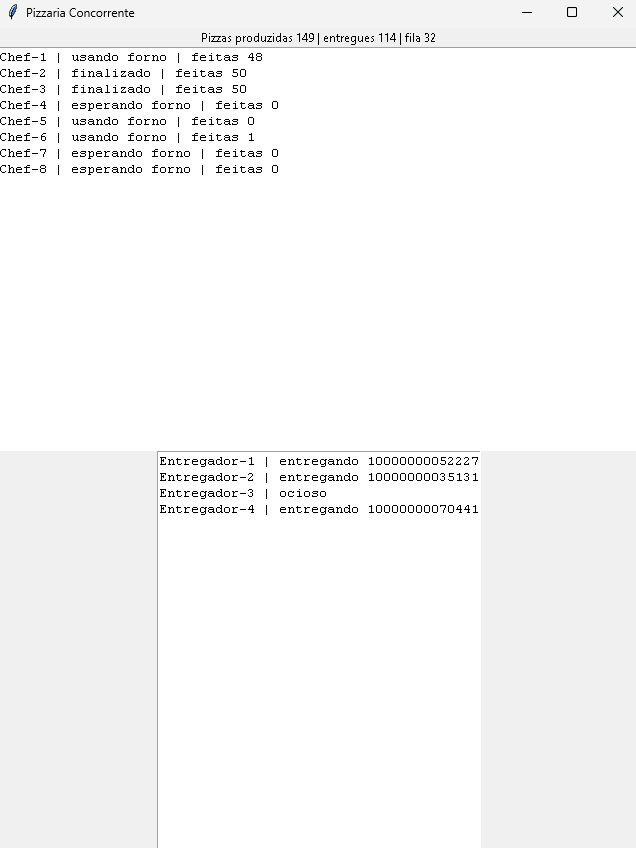
\includegraphics[width=0.9\textwidth]{fig1.png}
\caption{Execu\c{c}\~ao geral do sistema mostrando chefs, entregadores e a interface gr\'afica em funcionamento.}
\end{figure}

\begin{figure}[H]
\centering
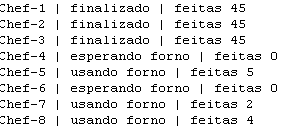
\includegraphics[width=0.9\textwidth]{fig2.png}
\caption{Situa\c{c}\~ao em que chefs est\~ao aguardando o forno, evidenciando o bloqueio causado pelo sem\'aforo.}
\end{figure}

\begin{figure}[H]
\centering
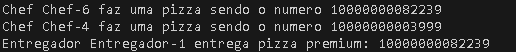
\includegraphics[width=0.9\textwidth]{fig3.png}
\caption{Situa\c{c}\~ao em que uma pizza fica pronta e ocorre a notifica\c{c}\~ao do consumidor via \texttt{Condition}.}
\end{figure}

\section{Etapa 3 -- Medi\c{c}\~ao e Gr\'afico}
O arquivo \texttt{graph.py} foi desenvolvido para automatizar a etapa de medi\c{c}\~ao. A ideia central \'e executar o programa com diferentes quantidades de threads, registrar o tempo total e comparar o ganho de desempenho.

Na vers\~ao atual, as medi\c{c}\~oes s\~ao realizadas nas quatro configura\c{c}\~oes pedidas pelo PDF: \(1\) chef + \(1\) entregador, \(2\) chefs + \(2\) entregadores, \(4\) chefs + \(4\) entregadores e \(8\) chefs + \(8\) entregadores.

Para que o gr\'afico de speedup represente de fato o efeito do paralelismo, todas as configura\c{c}\~oes processam a mesma carga total: 120 pizzas. Assim, a diferen\c{c}a entre os testes passa a ser a quantidade de threads utilizadas, e n\~ao o volume total de trabalho realizado.

Al\'em da exibi\c{c}\~ao em janela quando o backend do \texttt{matplotlib} permite, o script salva automaticamente a imagem do resultado em \texttt{grafico\_pizzaria.png}. Isso facilita a inclus\~ao do gr\'afico no relat\'orio mesmo em ambientes onde a interface gr\'afica do \texttt{matplotlib} n\~ao abre corretamente. O programa tamb\'em imprime no terminal uma tabela final com os valores exatos, o que ajuda no preenchimento da tabela do relat\'orio.

\subsection{M\'etrica utilizada}
O tempo total de execu\c{c}\~ao \'e medido em segundos, e o speedup \'e calculado pela express\~ao:
\[
S(N) = \frac{T(1)}{T(N)}
\]
em que \(T(1)\) representa o tempo da configura\c{c}\~ao de refer\^encia e \(T(N)\) representa o tempo medido para uma configura\c{c}\~ao com mais threads.

Nesse experimento, \(T(1)\) corresponde ao caso base com \(1\) chef e \(1\) entregador processando as mesmas 120 pizzas totais que ser\~ao distribu\'idas nas demais configura\c{c}\~oes.

\subsection{Tabela de resultados}
\begin{table}[H]
\centering
\begin{tabular}{cccc}
\toprule
\textbf{Configura\c{c}\~ao} & \textbf{Total de threads} & \textbf{Tempo total (s)} & \textbf{Speedup} \\
\midrule
1 chef + 1 entregador & 2 & 25.4753 & 1.0000 \\
2 chefs + 2 entregadores & 4 & 14.5719 & 1.7482 \\
4 chefs + 4 entregadores & 8 & 10.2249 & 2.4915 \\
8 chefs + 8 entregadores & 16 & 9.6462 & 2.6410 \\
\bottomrule
\end{tabular}
\caption{Tabela para registro dos tempos e speedups.}
\end{table}

Os resultados mostram que houve ganho de desempenho com o aumento do n\'umero de threads, mas sem crescimento linear perfeito. O melhor resultado observado foi na configura\c{c}\~ao com 8 chefs e 8 entregadores, que alcan\c{c}ou speedup de 2.6410 com 16 threads no total.

\begin{figure}[H]
\centering
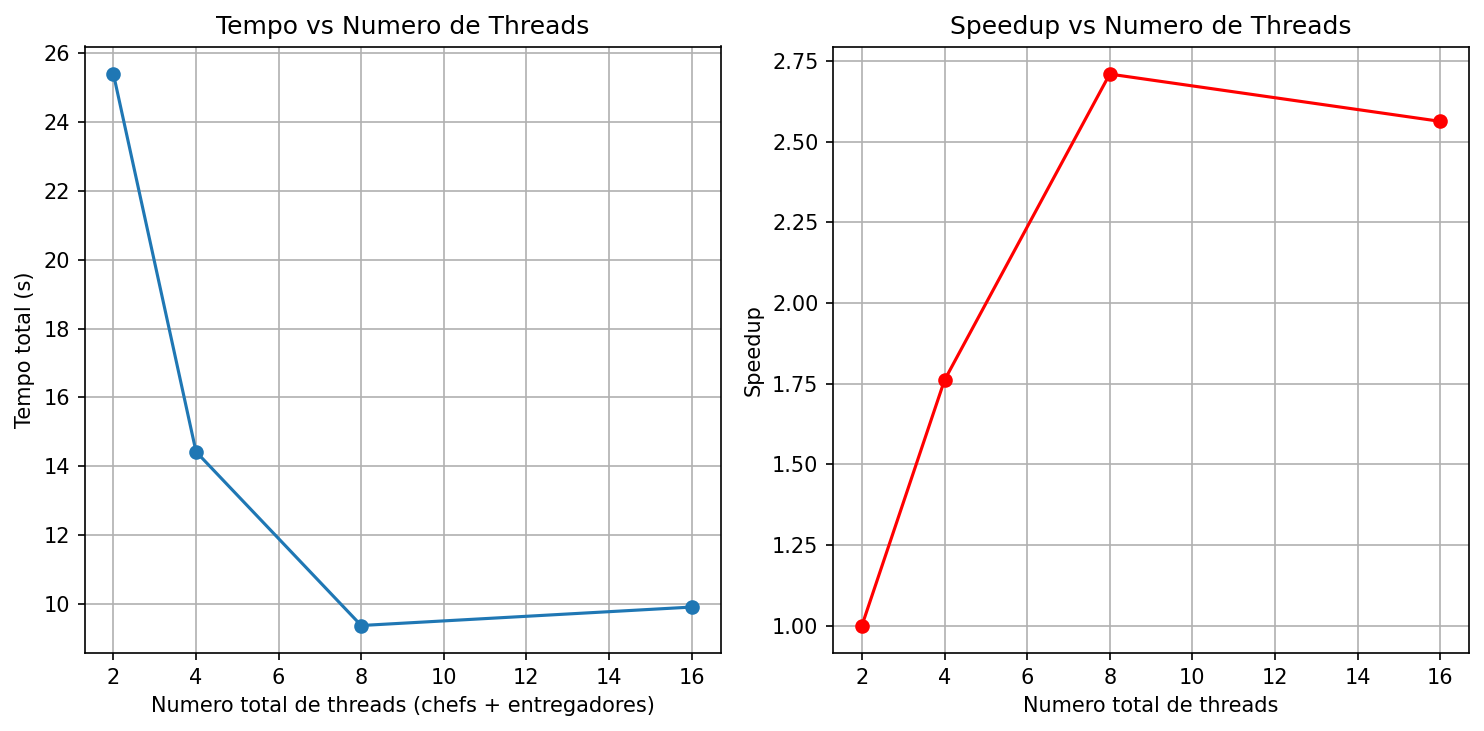
\includegraphics[width=\textwidth]{fig4.png}
\caption{Gr\'afico de tempo total e speedup gerado a partir do arquivo \texttt{graph.py}.}
\end{figure}

\section{Etapa 4 -- An\'alise pela Lei de Amdahl}
A Lei de Amdahl permite interpretar por que o speedup n\~ao cresce indefinidamente com o aumento do n\'umero de threads. Mesmo quando h\'a paralelismo, ainda existe uma fra\c{c}\~ao sequencial do programa, al\'em de custos extras de sincroniza\c{c}\~ao, conten\c{c}\~ao e troca de contexto.

A f\'ormula usada para estimar o limite te\'orico \'e:
\[
S(N) \approx \frac{1}{B + \frac{1-B}{N}}
\]
em que \(B\) representa a fra\c{c}\~ao sequencial do programa.

\subsection{Respostas da Etapa 4}
\begin{enumerate}
    \item \textbf{Observando seus resultados, o speedup continua crescendo linearmente at\'e 8 threads? Por qu\^e?}

    N\~ao. O speedup cresce com o aumento do n\'umero de threads, mas de forma sublinear. Pelos resultados obtidos, o speedup foi de 1.7482 com 4 threads totais, 2.4915 com 8 threads totais e 2.6410 com 16 threads totais. Isso mostra que houve ganho com paralelismo, por\'em com retorno decrescente. O crescimento deixa de ser linear porque parte do programa continua sequencial e porque surgem custos extras de sincroniza\c{c}\~ao, conten\c{c}\~ao no sem\'aforo do forno, acesso \`a fila compartilhada e troca de contexto entre threads.

    \item \textbf{Estime aproximadamente a fra\c{c}\~ao sequencial \(B\) usando dois pontos da tabela.}

    Aplicando a Lei de Amdahl, \(S(N) \approx \frac{1}{B + \frac{1-B}{N}}\). Para \(N = 8\) threads totais e \(S(8) = 2.4915\), obteve-se aproximadamente \(B \approx 0.316\). Para \(N = 16\) threads totais e \(S(16) = 2.6410\), obteve-se aproximadamente \(B \approx 0.337\). Fazendo uma estimativa m\'edia, temos \(B \approx 0.33\). Isso indica que cerca de um ter\c{c}o do comportamento total da aplica\c{c}\~ao permanece sequencial ou n\~ao se beneficia plenamente do paralelismo.

    \item \textbf{Se voc\^e tivesse um computador com 32 n\'ucleos, qual seria o speedup m\'aximo te\'orico esperado?}

    Considerando \(B \approx 0.33\), o speedup te\'orico para 32 n\'ucleos seria:
    \[
    S(32) \approx \frac{1}{0.33 + \frac{1 - 0.33}{32}} \approx 2.85
    \]
    Portanto, mesmo com muito mais n\'ucleos dispon\'iveis, o ganho n\~ao cresceria indefinidamente. O limite te\'orico absoluto, quando \(N \to \infty\), seria aproximadamente \(\frac{1}{0.33} \approx 3.03\), o que refor\c{c}a a ideia de satura\c{c}\~ao do speedup.

    \item \textbf{Cite pelo menos duas causas reais de overhead que apareceram na sua implementa\c{c}\~ao.}

    Entre os principais overheads observados est\~ao o GIL do Python, que limita o paralelismo efetivo em trechos CPU-bound como o teste de primalidade, e a conten\c{c}\~ao no sem\'aforo do forno, que restringe quantos chefs podem trabalhar simultaneamente. Tamb\'em houve custo de sincroniza\c{c}\~ao com \texttt{Queue} e \texttt{Condition}, al\'em de troca de contexto entre muitas threads concorrentes. Esses fatores ajudam a explicar por que o speedup n\~ao cresce de forma linear.
\end{enumerate}

\section{Etapa 5 -- Reflex\~ao Final}
O projeto mostra, de maneira pr\'atica, que concorr\^encia e paralelismo n\~ao significam ganho ilimitado de desempenho. Aumentar o n\'umero de threads pode melhorar a vaz\~ao at\'e certo ponto, mas tamb\'em introduz custos de coordena\c{c}\~ao e disputa por recursos limitados.

\subsection{Resposta final}
A principal li\c{c}\~ao desta atividade foi perceber que aumentar o n\'umero de threads n\~ao significa, automaticamente, obter ganho proporcional de desempenho. Na pr\'atica, o paralelismo sempre encontra limites impostos por trechos sequenciais, sincroniza\c{c}\~ao, conten\c{c}\~ao por recursos compartilhados e custos de gerenciamento das threads. O experimento da pizzaria mostrou isso claramente: o speedup aumentou at\'e certo ponto, mas depois os ganhos passaram a diminuir.

Outro aprendizado importante foi entender que medir desempenho exige comparar as mesmas condi\c{c}\~oes de trabalho. Quando a carga total foi mantida fixa, o gr\'afico passou a representar corretamente o efeito do paralelismo. Isso mostrou que a an\'alise de performance n\~ao depende apenas do c\'odigo, mas tamb\'em da forma como o experimento \'e planejado.

Esse tipo de satura\c{c}\~ao do speedup \'e especialmente cr\'itico em sistemas reais como servidores web de alta concorr\^encia, aplica\c{c}\~oes de processamento de dados, jogos e sistemas de machine learning. Nesses cen\'arios, muitas requisi\c{c}\~oes ou tarefas competem por CPU, mem\'oria, filas e regi\~oes cr\'iticas. Quando o projeto n\~ao considera esses gargalos, adicionar mais threads ou mais n\'ucleos pode trazer ganho pequeno, ou at\'e piorar o desempenho. Por isso, a principal conclus\~ao \'e que paralelizar bem significa equilibrar trabalho, reduzir overhead e conhecer os limites reais da arquitetura usada.

\section{Conclus\~ao}
O projeto est\'a bem organizado em m\'odulos e separa claramente as responsabilidades de inicializa\c{c}\~ao, concorr\^encia, interface e medi\c{c}\~ao experimental. O arquivo \texttt{main.py} coordena a execu\c{c}\~ao, \texttt{pizzaria.py} implementa o comportamento concorrente central, \texttt{interface.py} fornece visibilidade sobre o estado interno e \texttt{graph.py} viabiliza a an\'alise de desempenho.

Com isso, o c\'odigo atende \`a proposta did\'atica da atividade e fornece uma base s\'olida tanto para a demonstra\c{c}\~ao da concorr\^encia quanto para a an\'alise dos limites pr\'aticos do paralelismo.

\end{document}
